\documentclass[10pt]{article}
\usepackage[a4paper,textwidth=5.6in,textheight=9.1in,top=1.0in,headsep=.2in]{geometry}
\usepackage[T1]{fontenc}
\usepackage[utf8]{inputenc}
\usepackage{mathptmx}
\usepackage[scaled=.90]{helvet}
\usepackage{courier}
\usepackage{amsmath,amssymb,amsthm}
\usepackage{algorithm}
\usepackage{algpseudocode}
\newtheorem{definition}{Definition}
\usepackage{microtype}
\usepackage{booktabs,multirow,array,tabularx}
\usepackage{graphicx}
\usepackage[table]{xcolor}
\usepackage{tikz}
\usetikzlibrary{positioning,arrows.meta,fit,calc,backgrounds}
\usepackage[font=small,labelfont=bf,skip=4pt]{caption}
\usepackage{subcaption}
\usepackage{enumitem}
\usepackage[numbers,sort&compress]{natbib}
\usepackage[colorlinks=true,linkcolor=blue!50!black,citecolor=blue!50!black,urlcolor=blue!50!black]{hyperref}
\usepackage{fancyhdr}
\makeatletter\setlength{\@fptop}{0pt}\makeatother % float pages start at the top
\setlist{nosep,leftmargin=1.4em}
\definecolor{core}{HTML}{2A78D6}\definecolor{refl}{HTML}{EB6834}\definecolor{ink2}{HTML}{52514E}
\newcommand{\pp}{\,pp}
\newcommand{\ci}[2]{\,[#1,\,#2]}
\renewcommand{\topfraction}{.9}\renewcommand{\bottomfraction}{.8}\renewcommand{\textfraction}{.1}\renewcommand{\floatpagefraction}{.8}
\pagestyle{fancy}\fancyhf{}\renewcommand{\headrulewidth}{0pt}\fancyfoot[C]{\thepage}
\fancyhead[C]{\small\itshape Preprint.}
\newcommand{\GTWOREPL}{triples them on 300 fresh missions (4.3\,\% with the core, 14.7\,\% without)}
\newcommand{\GCONCL}{The slow feelings, trained on short episodes, do not yet replace an explicit energy rule.}
\newcommand{\GOPERATOR}{}
\newcommand{\GTHREE}{}
\newcommand{\GFOUR}{}


\title{\vspace{-.6em}\rule{\linewidth}{3pt}\\[.55em]\textbf{Feelings Learned from Consequences:\\ A Somatic-Marker Core for Language-Instructed Drone Missions,\\ and Where Language Models Do Not Help}\\[-.15em]\rule{\linewidth}{1pt}}
\author{\textbf{Mark Kolpakov}\\ Independent researcher\\ \texttt{markkolpakov96@gmail.com}}
\date{}

\begin{document}
\maketitle
\thispagestyle{fancy}

\begin{abstract}
Human decisions are guided by feelings: fast, compressed summaries of past consequences (Damasio's somatic markers).
We ask whether a machine can grow such feelings from consequences alone, whether acting on them makes a robot safer, and
whether a large language model (LLM) that makes decisions benefits from receiving them. A first study taught us a
methodological lesson that we document: when the researcher defines the feeling or the correct answer, a feeling written as
text carries everything, and words always tie with feelings. We therefore built a drone simulator in which every target comes
from the physics of the world. By forking an exact copy of the simulator we label, for every moment and for each of seven
candidate fast actions, whether a contact follows within 2\,s; homeostatic feelings (GPS distrust, being lost, low energy,
strain) are labelled from the true state. A small feeling core trained only on these consequences predicts contacts with the
static world with AUROC 0.91--0.92 in familiar and 0.86--0.87 in unseen places and, used as somatic markers over candidate
actions that include an efference copy of each candidate, cuts hits on the static world in closed-loop flight by 92\,\% and
85\,\% (familiar / unseen places, three seeds), whereas a classic reflex cuts them by 42\,\% and 22\,\%. In whole missions given as
free text plus a rough point in real OpenStreetMap places, under wind, GPS loss and spoofing and attacking birds, removing the
core doubles the missions with a static contact on 500 paired missions and \GTWOREPL. The slow feelings are weaker: in hard
missions with a weak battery, the battery died in the air in 29\,\% of missions with the learned ``low energy'' feeling and in
16\,\% with a plain energy-to-home rule over raw telemetry. The LLM results are mostly negative,
and we report them as such: feelings in words do not beat raw telemetry, words about the future of the world are ignored, and a
vision-language model does not single out a described target among look-alikes better than coordinates; the one clearly useful
language component is a small parser that turns the operator's request into a mission structure. We release the system,
including a bridge to the PX4 autopilot checked in software-in-the-loop, with an honest account of what is not yet ready for a
real aircraft.
\end{abstract}

\section{Introduction}
People decide with feelings long before they can name a rule. In the somatic-marker view \citep{damasio1994,bechara1994,bechara1997},
bodily signals summarise past consequences and bias choice; patients with ventromedial prefrontal damage keep their reasoning but
decide poorly and lack these anticipatory signals, although the evidence is debated \citep{dunn2006}. \citet{man2019} argued that
machines need homeostatic feelings of their own: perceptions of their body's deviation from a norm.

Language models now decide for agents and robots. Two-system robot architectures \citep{lin2023swiftsage,gr00t2025,helix2025}
pass \emph{intentions} top-down, from a slow model to a fast controller. We study the opposite direction: a small, fast core that
learns \emph{feelings} from consequences and passes them bottom-up to the slow decision-maker. We ask four questions:
(i)~Can a core learn useful feelings from the world's consequences alone, with no feeling set by hand?
(ii)~Does acting on them make a robot safer, in closed loop and in whole missions, in places it has never seen?
(iii)~Does an LLM decide better with the feelings than with the raw numbers they are computed from?
(iv)~Where in a language-instructed mission is a language model actually needed?

\paragraph{A lesson that shaped the design.} In the first phase of this project (\S\ref{sec:prelim}) every experiment in which
the researcher set the feeling, by a number or a rule, ended in a tie between words and feelings: a named feeling with an
intensity transmits losslessly as text, and a model trained on rule-made answers must learn the rule. The value of feelings in
humans lies elsewhere: speed, compression of many past consequences, learning from consequences rather than instructions, and
the state of one's own body. In the drone study every target therefore comes from the physics of the world or from human data.

\paragraph{What we call a feeling.} We use the word in the functional sense of \citet{man2019} and make no claim about experience.
A feeling is a calibrated probability, computed on board from the drone's own sensors, that a consequence the drone cannot yet
observe will happen: a contact within $h$ seconds if it keeps its current command, a GPS error above 5\,m, an own-position error
above 10\,m, an energy shortfall before the mission ends, or the motors at their limit. A somatic marker is the same probability for
a candidate action instead of the current command. The \emph{feeling core} is the small recurrent network that computes the
feelings (\S\ref{sec:method}, Definition~\ref{def:feeling}). Its targets are produced by forking an exact copy of the simulated world,
so no feeling and no correct answer is set by the researcher.

\paragraph{Contributions.}
\begin{itemize}
\item A protocol for learning feelings without a designer: consequence labels from forks of an exact simulator copy, strict
splits of places and threat families, decoys, an encounter generator, observability strata, three seeds and rules written
before each experiment (\S\ref{sec:sim}).
\item A feeling core whose somatic markers over candidate actions choose the fast action, with large and replicated safety gains
in closed loop and in whole missions in unseen real places (\S\ref{sec:fast}, \S\ref{sec:missions}).
\item Lesion experiments in the spirit of Damasio's patients: the whole core, single feelings, false and delayed feelings
(\S\ref{sec:stageg}).
\item A set of negative results on LLM decision-making with feelings, each stopped or judged by a pre-registered rule, and cheap
pilot tests that show \emph{before} any expensive training whether an LLM can matter at all (\S\ref{sec:slow}, \S\ref{sec:vlm}).
\item An end-to-end system, one request (text plus a rough point) to a finished mission, with a bridge to the PX4 autopilot and an
honest readiness assessment (\S\ref{sec:px4}).
\end{itemize}

\begin{figure}[t]
\centering
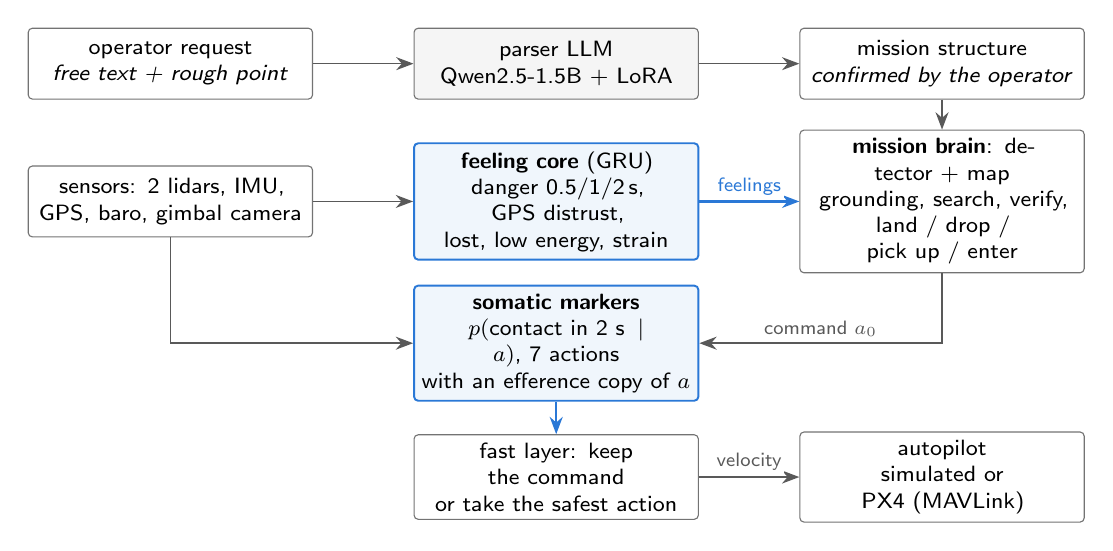
\begin{tikzpicture}[font=\sffamily\footnotesize,
  box/.style={draw=black!55, rounded corners=1.5pt, fill=white, align=center, inner sep=3pt, minimum height=9mm, text width=34mm},
  corebox/.style={box, draw=core, fill=core!7, line width=.7pt},
  llm/.style={box, fill=black!4},
  arr/.style={-{Stealth[length=2.2mm]}, line width=.6pt, black!65},
  carr/.style={-{Stealth[length=2.2mm]}, line width=.8pt, core},
  lab/.style={font=\sffamily\scriptsize, fill=white, inner sep=1pt}]
\node[box]  (req)   at (0,0)      {operator request\\ \emph{free text + rough point}};
\node[llm]  (parse) at (4.9,0)    {parser LLM\\ Qwen2.5-1.5B + LoRA};
\node[box]  (ms)    at (9.8,0)    {mission structure\\ \emph{confirmed by the operator}};
\node[box]  (sens)  at (0,-1.75)  {sensors: 2 lidars, IMU,\\ GPS, baro, gimbal camera};
\node[corebox](core)  at (4.9,-1.75){\textbf{feeling core} (GRU)\\ danger 0.5/1/2\,s, GPS distrust,\\ lost, low energy, strain};
\node[box]  (brain) at (9.8,-1.75){\textbf{mission brain}: detector + map\\ grounding, search, verify,\\ land / drop / pick up / enter};
\node[corebox](mark)  at (4.9,-3.55){\textbf{somatic markers}\\ $p(\text{contact in 2 s}\mid a)$, 7 actions\\ with an efference copy of $a$};
\node[box]  (fast)  at (4.9,-5.25){fast layer: keep the command\\ or take the safest action};
\node[box]  (ap)    at (9.8,-5.25){autopilot\\ simulated or PX4 (MAVLink)};
\draw[arr] (req) -- (parse); \draw[arr] (parse) -- (ms); \draw[arr] (ms) -- (brain);
\draw[arr] (sens) -- (core); \draw[arr] (sens.south) |- (mark.west);
\draw[carr] (core) -- node[lab, above=1pt]{feelings} (brain);
\draw[arr] (brain.south) |- node[lab, pos=.75, above=1pt]{command $a_0$} (mark.east);
\draw[carr] (mark) -- (fast); \draw[arr] (fast) -- node[lab, above=1pt]{velocity} (ap);
\end{tikzpicture}
\caption{System overview. The feeling core (blue) is trained only on consequences in the simulated world. Its slow feelings feed
the mission brain; its somatic markers evaluate the brain's velocity command and six alternatives and switch to the safest one when
``keep going'' becomes dangerous. Language enters only through the parser of the operator's request.}
\label{fig:arch}
\end{figure}

\section{Related work}
\paragraph{Somatic markers and feeling machines.} The hypothesis \citep{damasio1994,bechara1997} and its critique \citep{dunn2006}
motivate our lesion design; \citet{man2019} frame feelings as perceived homeostatic deviation. We use the idea as an engineering
hypothesis and test it ourselves.
\paragraph{Learning danger from one's own crashes.} \citet{gandhi2017} learned to fly by crashing a real drone 11,500 times;
\citet{lipton2016} trained an intrinsic-fear model of approaching catastrophes. Our core labels the \emph{counterfactual}
consequences of every candidate action by forking the simulator, adds homeostatic feelings, and passes them to an LLM.
\paragraph{Predicting collisions and future measurements.} DroNet \citep{loquercio2018dronet} predicts a collision probability from
a camera image, \citet{kahn2017uncertainty} learn collision prediction with uncertainty for safe exploration, and
\citet{dosovitskiy2017future} train agents to predict future measurements of their own state under candidate actions. Our somatic
markers are closest to the last: a learned prediction of a consequence for each candidate action. The differences are that every
label comes from a fork of an exact copy of the world rather than from the logged future of the one action taken, that homeostatic
feelings sit next to the danger feelings, and that we test whether a language model benefits from them.
\paragraph{Safety filters.} Shields \citep{alshiekh2018shield} and control barrier functions \citep{ames2019cbf} override a policy
when its action would leave a safe set given by a model or a formal specification. Our fast layer plays the same role but learns
the unsafe set from consequences, with neither a dynamics model nor a hand-written specification.
\paragraph{Emotion and homeostasis in reinforcement learning.} \citet{moerland2018} survey emotions in RL agents;
\citet{keramati2014} define reward as the reduction of homeostatic deviation. Neither connects to an LLM decision-maker.
\paragraph{Fast and slow robot architectures.} LLM planners for robots \citep{ahn2022saycan,vemprala2023chatgpt} choose
skills from language; SwiftSage \citep{lin2023swiftsage}, GR00T N1 \citep{gr00t2025} and Helix
\citep{helix2025} pass intent top-down; we pass feelings bottom-up and measure the reliance on them.
\paragraph{Reliance on non-text signals.} MM-SHAP \citep{parcalabescu2023} measures modality contributions; we instead
judge the reliance by its effect on decisions whose correct answers come from the world.

\section{Preliminary study: researcher-set affect gives false ties}\label{sec:prelim}
Before the drone we tested LLMs with affective signals on human data. Three findings carry over.
\emph{False ties:} all experiments in which the researcher defined the affective variable or the correct answer ended with
words equal to feelings. \emph{Perception decides:} a null result for vocal distress came from a weak encoder; CLAP
\citep{elizalde2023clap} recognised the emotion of unseen actors in 46\,\% of cases (8 classes) and WavLM-large
\citep{chen2022wavlm} in 77.6\,\% (6 classes). \emph{A feeling without a name:} on CREMA-D \citep{cao2014cremad}, with targets
from 2,443 human raters, emotion intensity (absent from the recogniser's vocabulary) was read better from the raw voice than from
emotion labels in all three seeds (mean correlation with raters 0.382 vs.\ 0.322; one-sided exact permutation test over three seeds per arm, $p=1/20=0.05$); given both, the
LLM leaned on the labels (0.336, two seeds). Personalised adaptation on real reactions did not beat a shared model on ESConv
\citep{liu2021esconv} or PRISM \citep{kirk2024prism}.

\section{Simulator and protocol}\label{sec:sim}
\paragraph{World.} MuJoCo physics \citep{todorov2012mujoco} with a PX4-like velocity controller and randomised physics (mass
$\pm$15\,\%, thrust $\pm$10\,\%, drag $\times$0.6--1.6). Real places from OpenStreetMap \citep{osm}: city centres, panel
districts, private houses, forest settlements, power-line corridors, a Texas suburb. The held-out test places, never used in
training or debugging, are a residential district of Tokyo and a district of Kazan. The drone's map may be wrong (missing
buildings, wrong heights, unmapped trees).
\paragraph{Sensors and faults.} Two Livox Mid-360-class lidars (one inverted; about 20k points per unit per 0.1\,s), a MEMS IMU
with bias random walk, barometer, GPS with multipath near walls, down rangefinder, optical flow, wind estimate, battery, link, and a
stabilised gimbal camera. Faults have real causes: GPS loss, freezing, degradation and spoofing (the fix walks away at 0.6\,m/s while
looking healthy); lidar range loss, blind sectors, spurious points; compass errors; IMU jumps; link loss.
\paragraph{Threats.} An encounter generator with six trajectory families (straight, ballistic, pursuit with a turn limit, zigzag,
chaotic, stopper), speeds 1--1000\,m/s, all directions, sizes 5\,cm--1.5\,m and a pre-drawn miss distance; birds with flapping wings,
flocks and diving hawks. Pursuit and chaotic families and several fault types appear \emph{only} in the unseen split.

\begin{table}[t]
\centering\small
\caption{Provenance of every target. No feeling and no correct answer is set by the researcher.}
\label{tab:prov}
\begin{tabularx}{\linewidth}{@{}lX@{}}
\toprule
Target & Where the correct answer comes from \\
\midrule
danger in 0.5 / 1 / 2\,s & an exact fork of the world keeps the current command; was there a contact? \\
GPS distrust & true horizontal GPS error $>5$\,m \\
lost & error of the drone's own position estimate $>10$\,m \\
low energy & battery left after the remaining mission at the current drain $<15$\,\% \\
strain & share of the next 2\,s at the motor limit or tilted $>30^\circ$ (fork) \\
marker of action $a$ & a fork executes candidate $a$ for 2\,s; was there a contact? \\
mission success, wrong target & the world: touchdowns, where the cargo landed, what hangs on the hook, the true track \\
\bottomrule
\end{tabularx}
\end{table}

\section{Method}\label{sec:method}
\subsection{Setting and notation}
Time is discrete with step $\Delta=0.1$\,s. At step $t$ the simulator holds the true state $s_t$ (pose, velocity, battery and the
world), the drone receives an observation $o_t$, and the mission brain proposes a velocity command $c_t$. The feeling core sees
\begin{equation}
x_t=\big[\phi(o_{\le t});\ \psi(c_t)\big]\in\mathbb{R}^{103},\qquad \tilde x_t=\mathrm{clip}\big((x_t-\mu)\oslash\sigma,\,-8,\,8\big),
\end{equation}
where $\phi$ holds 97 numbers from the drone's own sensors and perception (motion and its source, GPS quality and signs of
deception such as disagreement with dead reckoning, wind, battery, link, lidar distances per sector, looming rates per sector as in
the locust LGMD neuron \citep{gabbiani2002}, and the five most dangerous tracks of an occlusion-aware tracker), $\psi(c_t)$ is a
six-number efference copy \citep{vonholst1950} of the command about to be executed, and $\mu,\sigma$ are training-set statistics. No input is computed
from the true state.

\subsection{Targets from forks of the world}
Let $f$ be the simulator transition, $s_{t+1}=f(s_t,c_t,\xi_t)$ with random disturbances $\xi_t$. A \emph{fork} copies the world at
step $t$ and runs the copy forward under a fixed command. For a horizon $h\in\{0.5,1,2\}$\,s with the current command held,
\begin{equation}
y^{(h)}_t=\mathbb{1}\Big[\exists\,\tau\in\{1,\dots,h/\Delta\}:\ \kappa(\tilde s_{t+\tau})=1\Big],\qquad
\tilde s_t=s_t,\quad \tilde s_{t+\tau+1}=f(\tilde s_{t+\tau},c_t,\tilde\xi_{t+\tau}),
\end{equation}
where $\kappa$ indicates a contact of the airframe. The homeostatic targets come from the true state:
\begin{align}
y^{\mathrm{gps}}_t&=\mathbb{1}\big[\lVert g_t-p_t\rVert_{xy}>5\,\mathrm{m}\big], &
y^{\mathrm{lost}}_t&=\mathbb{1}\big[\lVert \hat p_t-p_t\rVert_{xy}>10\,\mathrm{m}\big],\\
y^{\mathrm{low}}_t&=\mathbb{1}\big[\,b_t-\bar r_t\,L_t/v<15\,\%\,\big], &
y^{\mathrm{strain}}_t&=\frac{1}{K}\sum_{k=1}^{K}\mathbb{1}\big[u_{t,k}\in\partial U\ \lor\ \vartheta_{t,k}>30^\circ\big],
\end{align}
with $g_t$ the GPS fix, $p_t$ the true and $\hat p_t$ the estimated position, $b_t$ the charge in per cent,
$\bar r_t=\max\{(b_0-b_t)/t,\ 0.02\}$ the mean drain so far in per cent per second, $L_t$ the remaining path, $v$ the cruise speed,
and the sum over the $K$ physics steps of the next 2\,s with the motor command $u$ at a limit or the tilt $\vartheta$ above
$30^\circ$. $y^{\mathrm{gps}}$ is masked when there is no fix. The somatic marker of a candidate action
$a\in\mathcal A=\{\text{keep},\text{hover},\text{climb},\text{descend},\text{left},\text{right},\text{back}\}$ comes from a fork that
executes $a$ for 2\,s:
\begin{equation}
y^{a}_t=\mathbb{1}\Big[\exists\,\tau\in\{1,\dots,2\,\mathrm{s}/\Delta\}:\ \kappa(\tilde s^{\,a}_{t+\tau})=1\Big].
\end{equation}
Targets are labelled at every third step of 40-s episodes. Table~\ref{tab:prov} lists their provenance.

\begin{definition}[Feeling, somatic marker]\label{def:feeling}
For a consequence target $y_{t,k}$ defined above, the feeling $k$ at step $t$ is the drone's estimate
$\hat y_{t,k}\approx P\big(y_{t,k}=1\mid o_{\le t},\,c_t\big)$, computed from its own observations only and calibrated, i.e.\
$P(y_{t,k}=1\mid\hat y_{t,k}=q)\approx q$. The somatic marker of a candidate action $a$ is
$m_t(a)\approx P\big(y^{a}_t=1\mid o_{\le t},\,a\big)$.
\end{definition}

\paragraph{Data.} The core is trained on 1,715 episodes of 40\,s (about 19 hours of flight) in the training places, validated on
285 and tested on 350 episodes in familiar places and 350 in unseen places with unseen threat families.

\subsection{The feeling core}
A GRU \citep{cho2014gru} maps the feature sequence to logits for the set $\mathcal K$ of seven feelings (danger in 0.5, 1 and
2\,s, GPS distrust, low energy, strain, lost):
\begin{equation}\label{eq:gru}
h_t=\mathrm{GRU}\big(h_{t-1},\ \mathrm{GELU}(W_{\mathrm{in}}\tilde x_t+b_{\mathrm{in}})\big),\qquad z_t=W_{\mathrm{out}}h_t+b_{\mathrm{out}}\in\mathbb{R}^{7},
\end{equation}
with a 96-unit GELU \citep{hendrycks2016gelu} input layer and $\dim h_t=128$. Training minimises a class-weighted binary cross-entropy over the labelled steps,
\begin{equation}
\mathcal L=-\sum_{t\in\mathcal T}\sum_{k\in\mathcal K} m_{t,k}\Big[w_k\,y_{t,k}\log\sigma(z_{t,k})+(1-y_{t,k})\log\big(1-\sigma(z_{t,k})\big)\Big],
\qquad w_k=\mathrm{clip}\Big(\frac{1-\pi_k}{\pi_k},\,1,\,20\Big),
\end{equation}
where $\pi_k$ is the positive rate of feeling $k$ in the training data and $m_{t,k}$ masks missing targets. We use AdamW
\citep{loshchilov2019adamw} (learning rate $2\cdot10^{-3}$, weight decay $10^{-4}$), 25 epochs and gradient clipping at 1, and keep
the epoch with the lowest validation log-loss. Each output is then Platt-calibrated \citep{platt1999} on validation flights of
training places, $\hat y_{t,k}=\sigma(\alpha_k z_{t,k}+\beta_k)$. On board the core runs in NumPy in under 1\,ms per step.

\subsection{Somatic markers and the fast layer}
A gradient-boosted classifier \citep{pedregosa2011} (300 trees of at most 31 leaves, learning rate 0.08) is fitted on pairs of a
state and a candidate action,
\begin{equation}
m_t(a)=\hat P\big(y^{a}_t=1\ \big|\ \tilde x_t,\ e_a,\ \eta_a(x_t)\big),
\end{equation}
where $e_a$ is a one-hot code of $a$ and $\eta_a(x_t)\in\mathbb{R}^6$ is the candidate's own efference copy: its velocity in the
heading frame, its speed, and the free distance and a lidar contact score along its direction. A second classifier $m'_t(a)$ of the
same kind is fitted only on dangerous moments ($y^{\mathrm{keep}}_t=1$) and only on the alternatives, so that it ranks them where
it matters. The fast layer keeps the brain's command unless continuing looks dangerous:
\begin{equation}
a_t=\begin{cases}\text{keep}, & m_t(\text{keep})<\theta,\\[2pt]
\arg\min_{a\in\mathcal A\setminus\{\text{keep}\}} m'_t(a), & \text{otherwise},\end{cases}
\qquad \theta=Q_{0.95}\big\{\,m_t(\text{keep})\ :\ y^{\mathrm{keep}}_t=0\,\big\},
\end{equation}
and an override is held for 0.6\,s. The threshold $\theta$ is the 95th percentile of the marker on safe validation moments, so
5\,\% of moments in which nothing would happen trigger an override. Algorithm~\ref{alg:fast} gives one step of the layer.

\begin{algorithm}[t]
\caption{One step of the fast layer (every 0.1\,s).}\label{alg:fast}
\begin{algorithmic}[1]
\Require brain command $c_t$; features $x_t$; threshold $\theta$; hold time $T_h=0.6$\,s; override end $t_u$
\State $\hat y_t\gets\sigma(\alpha\odot z_t+\beta)$ with $z_t$ from Eq.~\eqref{eq:gru} \Comment{feelings, read by the slow layer}
\State $m_t(\text{keep})$, $m'_t(a)$ for $a\in\mathcal A\setminus\{\text{keep}\}$ from the two classifiers
\If{$m_t(\text{keep})\ge\theta$ \textbf{and} $t>t_u$}
  \State $a^\star\gets\arg\min_{a\ne\text{keep}} m'_t(a)$;\quad $t_u\gets t+T_h$;\quad $c^{\mathrm{held}}\gets$ velocity command of $a^\star$
\EndIf
\State \Return $c^{\mathrm{held}}$ if $t\le t_u$, otherwise $c_t$
\end{algorithmic}
\end{algorithm}

\subsection{Slow decisions}
In whole missions the slow layer reads two feelings: if $\hat y^{\mathrm{lost}}>0.7$ for 3\,s the drone descends to re-localise (at
most twice), and if $\hat y^{\mathrm{low}}>0.8$ it gives up the remaining steps and returns. The telemetry baseline replaces both
feelings with explicit rules: return when
\begin{equation}
b_t<\hat r_t\Big(\frac{d^{\mathrm{home}}_t}{v}+60\,\mathrm{s}\Big)+5\,\%,
\end{equation}
with $\hat r_t$ the drain measured over the last 30\,s and $d^{\mathrm{home}}_t$ the distance home, and re-localise when the
particle spread exceeds 8\,m while the GPS trust is below 0.4. In the LLM study (\S\ref{sec:slow}) the correct option at a decision
is defined by forking the world under each option $o$ and ranking the outcomes lexicographically,
\begin{equation}
o^{*}_t=\arg\max_{o}\ \big(\neg\,\text{crash},\ \neg\,\text{empty in the air},\ \text{legs reached},\ \text{ends at home},\
-\lfloor d^{\mathrm{next}}/5\,\mathrm{m}\rfloor\big),
\end{equation}
where $d^{\mathrm{next}}$ is the remaining distance to the next waypoint; 5-m bins make smaller gaps ties.

\subsection{Statistics}
Every comparison is paired: two variants fly the same missions with the same seeds, failures and threats. For an outcome $Y_i$ of
mission $i$ (for instance $\mathbb{1}[\text{static contact}]$) we report the mean paired difference and a 95\,\% percentile bootstrap
interval \citep{efron1993} over missions,
\begin{equation}
\hat\Delta=\frac1N\sum_{i=1}^{N}\big(Y^{A}_i-Y^{B}_i\big),\qquad
\mathrm{CI}_{95}=\big[\hat\Delta^{*}_{(2.5)},\ \hat\Delta^{*}_{(97.5)}\big],
\end{equation}
where $\hat\Delta^{*}_{(q)}$ is the $q$-th percentile of $\hat\Delta$ over $2000$ resamples of the missions. Single rates get the
same bootstrap; for rare events such as touching a wrong target, where the percentile bootstrap is optimistic, we also give
the exact Clopper--Pearson interval \citep{clopper1934}. Prediction quality is the area under the ROC curve (AUROC) and under the precision-recall curve (AUPRC);
calibration is the expected calibration error \citep{naeini2015,guo2017} over ten equal-width bins $B_1,\dots,B_{10}$ of the predicted probability,
\begin{equation}
\mathrm{ECE}=\sum_{b=1}^{10}\frac{|B_b|}{n}\,\Big|\,\frac{1}{|B_b|}\sum_{t\in B_b}\hat y_t-\frac{1}{|B_b|}\sum_{t\in B_b}y_t\,\Big|.
\end{equation}
Hypotheses, thresholds and stopping rules were written down
before each run.

\section{Fast feelings}\label{sec:fast}
\begin{table}[t]
\centering\small
\caption{What the core knows: AUROC of ``contact within 2\,s'' (familiar / unseen places; three seeds, spread $\le0.01$).}
\label{tab:auroc}
\begin{tabular}{@{}lccc@{}}
\toprule
Core & Static world & All contacts & Encounters \\
\midrule
Tracker rule & 0.54 / 0.54 & 0.53 / 0.54 & 0.52 / 0.54 \\
Memory-less (logistic) & \textbf{0.92} / 0.86 & 0.73 / 0.71 & 0.55 / 0.56 \\
GRU with memory & 0.91 / \textbf{0.87} & \textbf{0.74} / \textbf{0.72} & \textbf{0.58} / \textbf{0.57} \\
\bottomrule
\end{tabular}
\end{table}

\begin{table}[t]
\centering\small
\caption{The seven feelings on the test episodes (familiar / unseen places): base rate of the event, AUROC, AUPRC and expected
calibration error. Mean of three seeds; the standard deviation is at most 0.02 for AUROC and AUPRC and 0.006 for ECE. The danger
feelings count every contact, including physically unavoidable encounters.}
\label{tab:feelings}
\setlength{\tabcolsep}{4pt}
\begin{tabular}{@{}lcccc@{}}
\toprule
Feeling & Base rate & AUROC & AUPRC & ECE \\
\midrule
danger in 0.5\,s & 0.016 / 0.025 & 0.79 / 0.77 & 0.19 / 0.20 & 0.002 / 0.004 \\
danger in 1\,s & 0.032 / 0.050 & 0.78 / 0.76 & 0.23 / 0.25 & 0.005 / 0.007 \\
danger in 2\,s & 0.062 / 0.094 & 0.74 / 0.72 & 0.25 / 0.28 & 0.010 / 0.012 \\
GPS distrust & 0.132 / 0.174 & 0.94 / 0.81 & 0.65 / 0.41 & 0.009 / 0.041 \\
lost & 0.041 / 0.052 & 0.97 / 0.81 & 0.68 / 0.62 & 0.006 / 0.012 \\
low energy & 0.195 / 0.219 & 0.99 / 0.99 & 0.96 / 0.96 & 0.015 / 0.014 \\
strain & 0.223 / 0.317 & 0.99 / 0.99 & 0.97 / 0.98 & 0.005 / 0.007 \\
\bottomrule
\end{tabular}
\end{table}

All seven feelings are informative and calibrated on unseen places (Table~\ref{tab:feelings}): AUROC 0.72--0.99 and ECE at most
0.041. The homeostatic feelings are the easiest to learn; the danger feelings are harder because many encounters are unavoidable.
Restricted to the static world, ``danger in 2\,s'' reaches AUROC 0.91 / 0.87 (Table~\ref{tab:auroc}). At 5\,\% false alarms the core
warns of 93\,\% / 89\,\% of static contacts, on average 1.1--1.2\,s ahead.
Observability strata order the encounter feeling exactly as a sensor would: visible to the lidar now 0.74, avoidable by physics 0.64,
within 40\,m but unseen 0.60, unavoidable 0.57, beyond range 0.52. When danger is known, the consequence model with a choice model
picks a safe action in 0.498$\pm$0.003 / 0.394$\pm$0.002 of cases, above the best fixed reaction chosen in hindsight
(0.455 / 0.352) and the lidar geometry heuristic (0.298 / 0.257).

\begin{figure}[t]
\centering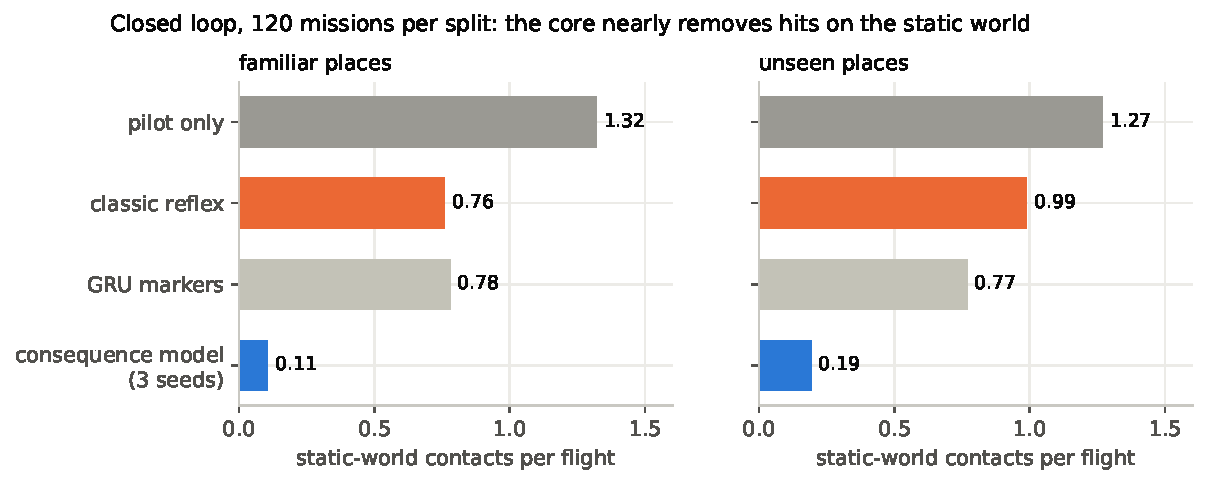
\includegraphics[width=\linewidth]{fig_closed_loop.pdf}
\caption{Closed loop, 120 missions per split, the same missions for every fast layer. Static-world contacts per 40-s flight.
The somatic-marker core (blue; mean of three seeds) nearly removes hits on the static world in familiar and unseen places.}
\label{fig:closed}
\end{figure}

\paragraph{Closed loop.} Over the same 120 missions per split (Fig.~\ref{fig:closed}), the somatic-marker core reduces static
hits by 92\,\% (familiar) and 85\,\% (unseen) and all contacts by 67\,\% and 54\,\% (mean of three seeds). Paired against the classic
reflex the difference is $-0.77$\ci{-1.06}{-0.50} and $-0.77$\ci{-1.07}{-0.49} contacts per flight. The core was trained on data
from a pilot that, by a bug found later, hovered after its first pause; it flies with the corrected pilot, a transfer to a different
behaviour. The cost is 12--13\,\% of mission progress per 40\,s; encounter hits barely change, as most are physically unavoidable.

\section{Slow decisions: the core decides, the LLM adds nothing}\label{sec:slow}
At five moments of a 120-s flight (about 12, 30, 48, 66 and 84\,s, each jittered by $\pm2$\,s) the drone chooses among continue,
climb and continue, wait 10\,s, land now and go home; the best option is defined by forks of the world (\S\ref{sec:method}). We fine-tuned Qwen2.5-1.5B \citep{qwen25} with LoRA \citep{hu2022lora} (rank 16, $\alpha=32$, dropout 0.05 on all
attention and MLP projections; AdamW at $2\cdot10^{-4}$, 8 epochs for every variant) on seven inputs, three seeds each, with
shuffled answer order (Fig.~\ref{fig:llm}). Every prompt states the time in the air, the legs left, the remaining path and the
distance home. Variant N adds nothing else; T adds the raw telemetry in words (GPS satellites and HDOP, time and distance without a
good fix, the velocity source, battery, altitude, speed, wind); F adds the seven feelings as percentages; FT adds both. In the slot
variants the feeling logits (Fs) or the eleven telemetry numbers (Ts) pass through a small MLP (64 GELU units) into four input
embeddings of the LLM, trained at $10^{-3}$; FsT combines feeling slots with telemetry in words.
\begin{figure}[t]
\centering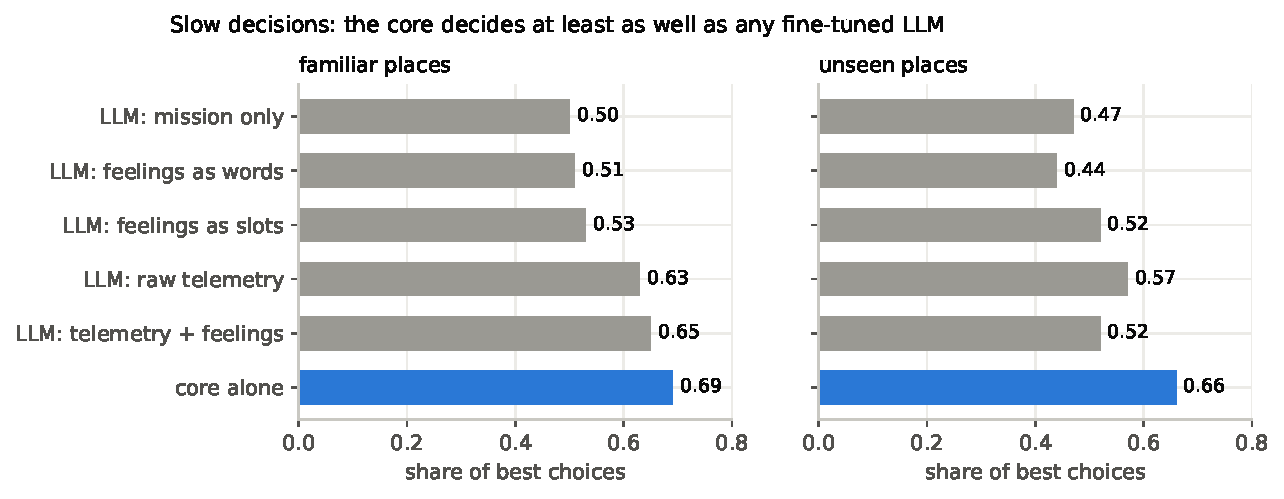
\includegraphics[width=\linewidth]{fig_llm_decisions.pdf}
\caption{Slow decisions: share of best choices (mean of three seeds). The core alone (a small policy on feelings and telemetry)
decides at least as well as any fine-tuned LLM. Feelings written as words do not beat raw telemetry.}
\label{fig:llm}
\end{figure}
Feelings in words did not beat raw telemetry (FT$-$T: $+0.02$\ci{-0.03}{0.07} familiar, $-0.05$\ci{-0.11}{0.01} unseen);
feelings fed as soft embedding slots did beat the same feelings in words on unseen places ($+0.08$\ci{0.03}{0.13}) and the
slot models relied on the low-energy feeling (inverting it cost 0.10--0.12). Handing the LLM the decisions the core was least sure
about only hurt (0.69$\to$0.63 when all were handed over). Messages in words about the future of the world (wind fronts, GPS
jamming, cold; 25\,\% false) were ignored: removing them from a trained model changed nothing ($0.00$\ci{-0.01}{0.01}). An LLM
given the core's per-option judgement trusted it strongly (swapping it cost 0.16--0.26) and all six such models trained stably,
whereas four of six trained on raw numbers collapsed to a constant answer. A third stage with strong events was stopped by its
pre-registered pilot rule: the announced event changed the best plan in only 15\,\% of decisions (threshold 20\,\%), a test that
took ten CPU minutes instead of hours of GPU training.

\section{Who picks the target? A vision-language model vs.\ geometry}\label{sec:vlm}
In 400 scenes with look-alikes (70\,\% containing a twin of the same kind and colour), Qwen2.5-VL-7B \citep{qwen25vl} zero-shot
boxed the described target in 0.19 of hard visible scenes, below ``nearest to the rough point'' (0.38) and chance (0.34); with
numbered marks \citep{yang2023som} it reached 0.41--0.46 and with close-ups of every candidate 0.50\ci{0.42}{0.58}. A sentence encoder with perfect
perception reached 0.69 on novel wording. The VLM was robust to new wording but could not separate twins by size and relations;
the pre-registered rules failed and no closed loop with a VLM was built.

\section{Whole missions from one request in real places}\label{sec:missions}
\paragraph{System.} The operator's text becomes a mission structure through Qwen2.5-1.5B + LoRA (the same LoRA settings, two epochs) trained on templates and 4,591
paraphrases by Qwen2.5-7B with a meaning back-check; it is exact on 56\,\% of 100 hand-written Russian tasks (threshold 85\,\%), so
the operator confirms the parse in the app. A YOLO11s detector \citep{yolo11} trained on segmentation-labelled frames of training
places reaches recall 0.974 and precision 0.978 on the test places (colour 0.958). Grounding is geometric: relations are computed
over the map and the detections; descriptions follow \citet{dale1995}. Navigation fuses dead reckoning, lidar-inertial odometry and a
lidar-to-map particle filter (without GPS 0.25--0.8\,m error over a 1.2\,km route at 25--30\,m). A state machine flies over the
mapped roofs, searches, looks closer, checks every stated attribute up close before touching anything, acts and returns. A
touching action (land, drop, pick up, enter) is executed alone only for an \emph{unambiguous} target; otherwise the drone asks the
operator or skips the step.

\paragraph{F4--F5 (500 missions in the held-out places; GPS loss planned in 187 and reached before the mission ended in 175, bird attacks in 256, wind with gusts).}
The first pre-registered run failed its safety rule (wrong target 3.2\,\%, rule $\le$2\,\%); after the unambiguous-target rule and
fixes found by reading flight traces, the wrong-target rate fell to 1.6\,\% and then 0.67\,\%\ci{0}{1.67} (exact Clopper--Pearson upper bound 2.4\,\%; Table~\ref{tab:f4}).
Removing the core (classic reflex instead of somatic markers) raised the missions with a static contact from 5.4\,\% to 11.0\,\%,
$-0.28$\ci{-0.48}{-0.11} static contacts per mission, and in the 173 missions where GPS was lost in both runs from 0.25 to 0.77 per mission. Against attacking birds the
core was no better than the reflex. Replacing the slow feelings by raw telemetry made no difference, but those feelings almost never
fired in these short missions (``lost'' in 23 of 500, ``low energy'' in 2); \S\ref{sec:stageg} tests them where they should matter.

\begin{table}[t]
\centering\small
\caption{Whole missions in unseen places. F4 is the first pre-registered run; F4b and F4d are post-hoc fixes of the same system,
reported as such. Brackets: 95\,\% bootstrap intervals over missions. The F4 rule bounds the rate itself; the stage G rule
bounds the upper end of its interval.}
\label{tab:f4}
\begin{tabular}{@{}lccc@{}}
\toprule
 & F4 (500) & F4b (500) & F4d (300) \\
\midrule
Steps done & 0.289 & 0.266 & 0.322 \\
Wrong target (rule $\le$2\,\%) & 3.2\,\%\ci{1.8}{4.8} & 1.6\,\%\ci{0.6}{2.8} & 0.67\,\%\ci{0}{1.67} \\
Missions with a static contact & 5.0\,\% & 5.4\,\% & 3.3\,\% \\
\bottomrule
\end{tabular}
\end{table}

\section{Final test and lesions on fresh missions}\label{sec:stageg}
All parts of this stage were written down with their thresholds before the runs (stage G). The test places are the same held-out
Tokyo and Kazan districts, but the 300 missions are new: new layouts, new texts, new rough points, new failures. Nothing in the
system was tuned on them.

\paragraph{The final test (G2).} Table~\ref{tab:g2} gives the system alone (the operator's text parsed by the F3b parser, no person
to answer questions) and the same system with the classic reflex in place of the feeling core, on the same 300 missions.
The main result of the project repeats on this fresh set and is larger than before: without the core, 14.7\,\% of missions touch the
static world, with it 4.3\,\% (paired difference $-10.3$ percentage points\ci{-14.7}{-6.0}; $-0.61$\ci{-0.92}{-0.35} contacts per
mission). For the first time the core also reduces hits by attacking birds ($-0.19$\ci{-0.33}{-0.06} per attacked mission), and
the system with the core completes more steps ($+0.038$\ci{0.008}{0.070}). The pre-registered safety rule was not met: the drone
alone touched a wrong target in 3 of 300 missions, 1.0\,\% with a bootstrap upper bound of 2.3\,\% (exact Clopper--Pearson bound 2.9\,\%) against the required 2\,\%. Fig.~\ref{fig:lesion}
puts this replication next to the first lesion study.

\begin{table}[t]
\centering\small
\caption{Final test on 300 fresh missions in unseen places (G2). Same missions for both variants; brackets are 95\,\% bootstrap
intervals over missions. The difference column is paired.}
\label{tab:g2}
\setlength{\tabcolsep}{3.5pt}
\begin{tabular}{@{}lccc@{}}
\toprule
 & Feeling core (alone) & Classic reflex & Difference \\
\midrule
Missions with a static contact & \textbf{4.3\,\%}\ci{2.3}{6.7} & 14.7\,\%\ci{10.7}{18.7} & $-10.3$\ci{-14.7}{-6.0}\,pp \\
Static contacts per mission & & & $-0.61$\ci{-0.92}{-0.35} \\
Attack hits per attacked mission & & & $-0.19$\ci{-0.33}{-0.06} \\
Steps done & 0.301\ci{0.254}{0.348} & 0.257\ci{0.214}{0.304} & $+0.038$\ci{0.008}{0.070} \\
Whole missions done & 0.287\ci{0.233}{0.340} & 0.253\ci{0.207}{0.303} & $+0.033$\ci{0.003}{0.063} \\
Wrong target (rule $\le 2$\,\%) & 1.0\,\%\ci{0}{2.3} & 2.3\,\%\ci{0.7}{4.0} & $-1.3$\ci{-3.0}{-0.3}\,pp \\
\bottomrule
\end{tabular}
\end{table}

\begin{figure}[t]
\centering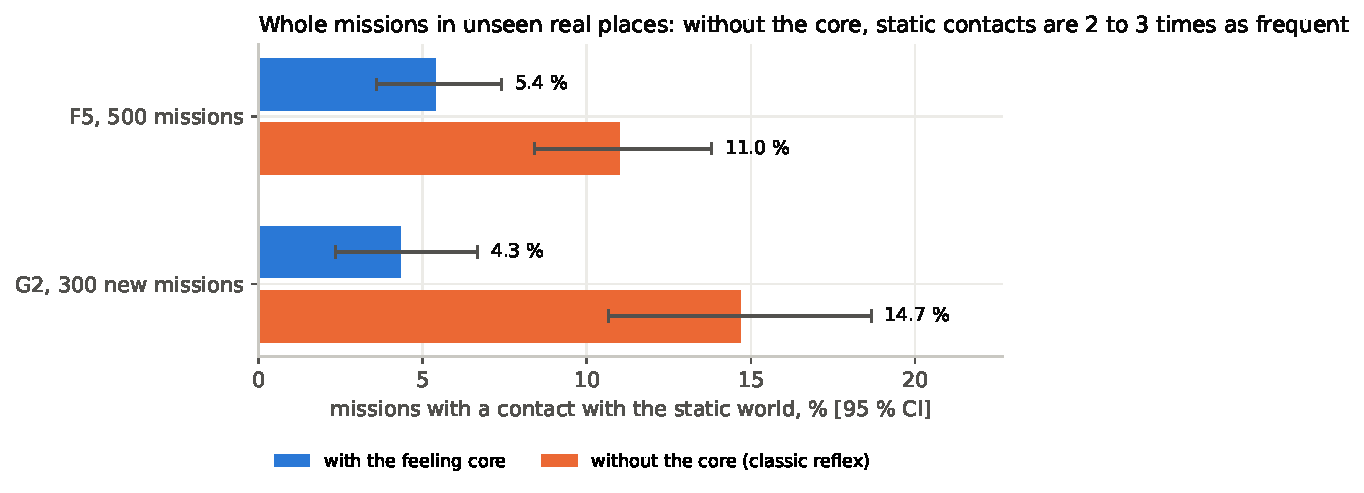
\includegraphics[width=.92\linewidth]{fig_missions_lesion.pdf}
\caption{Whole missions in unseen real places, with the feeling core and with a classic reflex in its place. F5: the first lesion
study (500 missions); G2: 300 fresh missions. Intervals: 95\,\% bootstrap over missions.}
\label{fig:lesion}
\end{figure}

\paragraph{Alone and with an operator.} By action, the drone alone completed fly-by in 0.49 of steps, landing 0.44, inspection 0.30,
hook pick-up 0.29, parachute drop 0.22 and hangar entry 0.14. Most failures are refusals by design: when the description
does not single out one object, the drone does not touch any. The app is meant to be used with a person who checks the parse and
answers the drone's questions, so we flew the first 200 missions once more that way. The simulated operator gets the true parse
and, when asked, picks the candidate view that lies at the meant object. On the 182 missions that finished within the run's time
limit (18 were still flying), the drone with an operator completed 0.56 of steps against 0.29 alone on the same missions (paired
$+0.27$\ci{0.20}{0.33}) and 0.54 of whole missions against 0.29 (Fig.~\ref{fig:actions}). Most missions needed no question at all
(median 0, 90th percentile 1). The help has a cost: the drone now flies every step to the end, and missions with a static contact
rose from 3.8 to 10.4\,\% ($+6.6$\ci{2.7}{10.4} points). It touched a wrong target in 4 missions (2.2\,\%); two of them are the
same mistakes it made alone, without asking. In three missions, when none of its candidates was the target, the drone asked again
and again (131 to 541 times): the app needs a limit there.

\begin{figure}[t]
\centering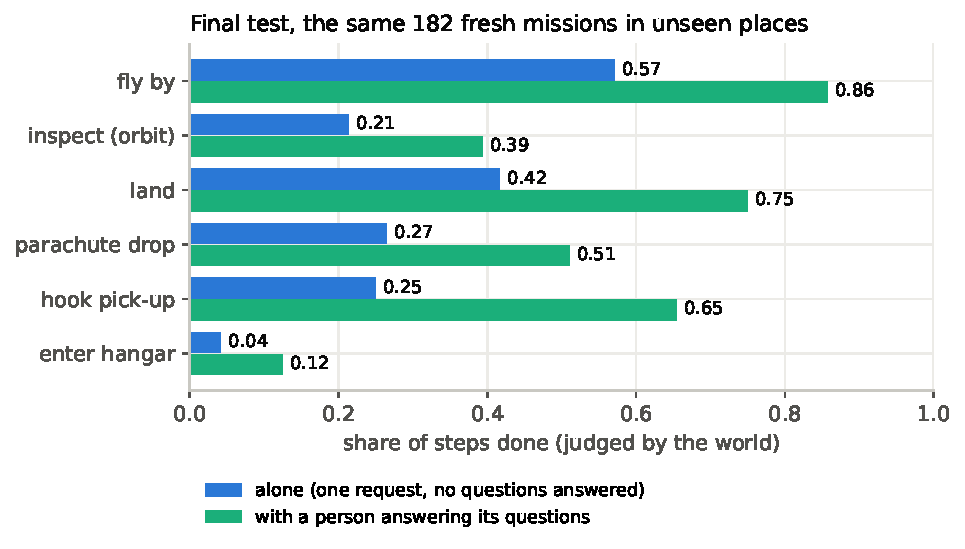
\includegraphics[width=.8\linewidth]{fig_actions.pdf}
\caption{Steps done by action on the same 182 fresh missions, by the drone alone and with a person who checks the parse and answers
its questions. Judged by the world: what it landed on, where the parcel fell, what hangs on the hook.}
\label{fig:actions}
\end{figure}

\paragraph{The hangar door (G1).} Hangar entry was the weakest action, and one traced failure showed the door finder taking a gap
in the back wall for the door. We tried a stricter rule: an opening counts only if the lidar sees the hangar's floor through it.
With the drone placed on the circle around 90 hangars, the old finder found the right door of 74 of 76 open hangars and no door in
any of 14 closed ones; the new one found 72, missed 4, and saw a door in 3 closed hangars. In flight, with the true parse and a
person answering the drone's questions, the new finder entered 1 hangar in 38 flights and the old one 6 in 37: the drone's own
position drifts while it circles, and the drift smears wall points across the box. By the rule written beforehand the old finder
stays.

\paragraph{Slow feelings in hard missions (G3).} The slow feelings (``I am lost'', ``low energy'') hardly ever fired in the short
missions of F5, so stage G tested them where they should matter. The 120 hard missions in the test places start with 30--65\,\%
charge, have a cold battery in 60\,\% of missions, wind of 3--9\,m/s, a lost GPS (47 of the 99 missions flown) or a spoofed one (26), bird attacks, and always require
the return home. The parse is true, so only the slow layer is tested. Five variants flew the same missions: the core's feelings;
raw telemetry with thresholds instead, which compares the charge with the energy needed to fly home; no slow layer; and each
feeling removed in turn. The time cut left 99 missions (98 for three variants; Fig.~\ref{fig:slow}).

With the core's feelings the battery died in the air in 29\,\% of missions, and without any slow layer also in 29\,\% (paired
difference $0.0$\ci{-7.1}{7.1} points). The first expectation, that the slow layer prevents such falls, is not confirmed. Raw
telemetry did better: 16\,\% falls ($-13.1$\ci{-21.2}{-5.1} points against the feelings) and more landings at home (63 against
52\,\%, $+11.1$\ci{5.1}{18.2}). It paid with fewer whole missions ($-0.040$\ci{-0.081}{-0.010}) because it turned home early twice
as often. H6 is therefore not confirmed, as we had written down beforehand: the ``low energy'' feeling was trained on 40-s
episodes and does not know the distance home, while the telemetry rule multiplies the drain by that distance. The feeling did act
(with it the drone turned home early in 13\,\% of missions, without it never), but the falls did not change ($0.0$\ci{-6.1}{6.1}).
Removing ``I am lost'' changed neither falls nor returns. One observation was not planned: without ``I am lost'' the drone touched
the static world less ($-0.22$\ci{-0.43}{-0.06} contacts per mission). For a real aircraft the lesson is plain. The energy reserve
must come from an explicit rule over distance and drain, not from a learned feeling.

\begin{figure}[t]
\centering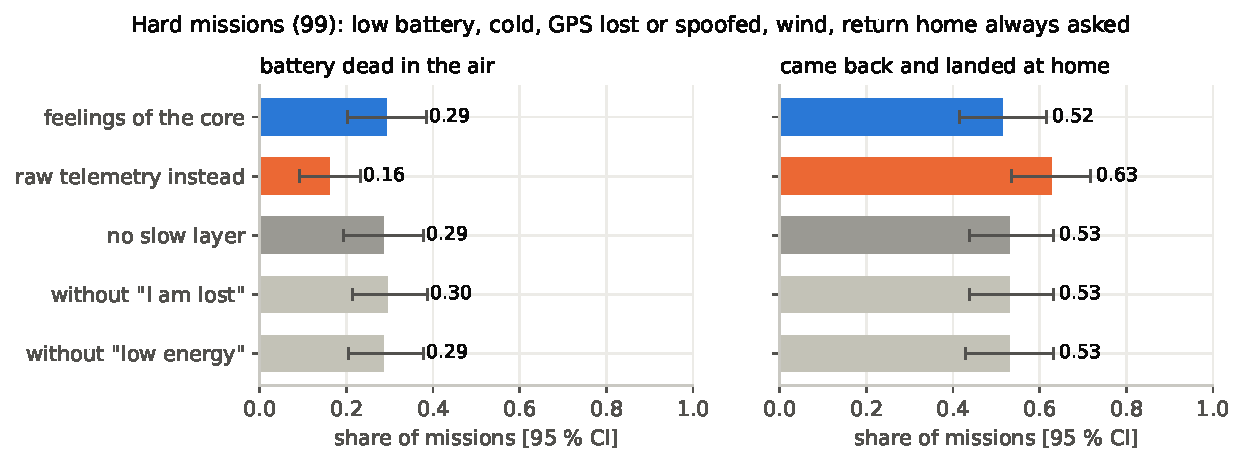
\includegraphics[width=\linewidth]{fig_slow.pdf}
\caption{Hard missions (G3), the same missions for all variants. Left: missions in which the battery died in the air. Right:
missions that ended with a landing at home. Raw telemetry with an energy-to-home rule beats the learned slow feelings; removing
the slow layer or a single feeling changes nothing. Intervals: 95\,\% bootstrap over missions.}
\label{fig:slow}
\end{figure}

\paragraph{False and delayed feelings (G4).} Damasio's patients suggest two more lesions: a feeling that fires when nothing is
there, and one that comes too late. On the first 100 missions of the final test we flew the full system twice more. In the first
variant the ``keep going'' marker reported danger in an empty sky for 1\,s at random moments, about once every 20\,s; in the
second the markers saw the world 0.3\,s late. False alarms added 24 overrides per mission\ci{19}{29} and did not cost steps
($+0.015$\ci{-0.05}{0.08}), but missions with a static contact rose from 4 to 9\,\% ($+5.0$\ci{0.0}{10.0} points): a needless
swerve in a street can itself end in a wall. We had expected fewer steps and no fewer contacts; the second half held, the first did
not. A 0.3-s delay changed little: missions with a static contact $+3.0$\ci{-1.0}{8.1} points, so the expected rise is not
confirmed. The markers look 2\,s ahead, and a 0.3-s lag is small against that horizon.

\subsection{Towards a real aircraft: the brain on the PX4 flight stack}\label{sec:px4}
A drone flies on an autopilot, not on our simulator's controller. We wrote a MAVLink bridge that gives the unchanged mission brain
the same interface on a real autopilot (PX4 \citep{meier2015px4} or ArduPilot): telemetry in, velocity set-points out at 20\,Hz, frame conversions, a
watchdog that holds position when the brain is slow, and the autopilot's own failsafes underneath. We then flew 12 missions
(landing, drop, pick-up, inspection, fly-by, ground-level targets) with PX4's software-in-the-loop build and its SIH quadrotor
model, posing our world at PX4's estimated pose every 0.1\,s so that the lidar, the camera and the scoring stay ours. The bridge
worked mechanically: PX4 armed, took off, flew the brain's commands, landed, re-armed and refused to arm when its simulated
sensors failed. Mission success did not transfer: 1 of 12 missions with PX4 against 7 of 12 with our controller on the same
missions, and holding position through PX4's own position loop in the precise phases did not change the count. PX4 tracks the
brain's velocity commands with a median error of 0.8--1.3\,m/s and missions took about twice as long. The brain's timeouts, speeds and
precision phases were tuned on our controller; they must be re-tuned and re-tested on the real flight stack before any flight.


\section{Discussion}
\paragraph{What the feelings are good for.} A core that compresses thousands of forked consequences into a calibrated ``if I keep
going, I hit something'', and evaluates each candidate action through its efference copy, is a strong fast controller. Its gains
survive unseen places, a changed pilot, three seeds, whole missions with perception and language in the loop, and a fresh mission
set. This is the clearest positive result of the project and a machine analogue of Damasio's lesion test: remove the core, keep all
raw data and a classic reflex, and missions with a static contact become 2.0 (F5) and 3.4 (G2) times as frequent.
\paragraph{Where the LLM helps and where it does not.} In our tasks the LLM was useful exactly once: turning a free-form request
into a mission structure. For decisions that the numbers decide, fast or slow, a small core decides at least as well; LLMs given the
core's judgement trust it and learn stably but add no value; words about the future were ignored; and a 7B VLM did not find a
described object among twins. We read this as a boundary rather than a failure: language matters where the \emph{goal} is in language.
\paragraph{Methodological lessons.} (1) Never let the researcher set the feeling or the answer. (2) A cheap pilot with world forks
tells whether an LLM \emph{can} matter before any expensive training. (3) Many of our early ``results'' were bugs: a tracker that was
99.6\,\% clutter, a pilot hovering after its first pause, a scorer that ignored the hangar floor, an autopilot without a horizontal
integrator stalling a metre short in 7\,m/s wind, a loop of 613 operator questions. Each was found by reading traces, not averages.

\section{Limitations}
All results are in simulation (MuJoCo, synthetic images); perception is trained on synthetic frames and will need real images.
The slow feelings were trained on 40-s episodes and do not know the distance home; in hard missions a telemetry rule beat them
(\S\ref{sec:stageg}). Small birds are a sensor limit. A second simulator
was planned but not done. The parser is below its thresholds. Budget limits forced smaller runs than planned in places. The PX4 check
co-simulates the flight stack with our world and shows that the mission brain, tuned on our own autopilot model, loses much of its
performance on PX4 without re-tuning (\S\ref{sec:px4}). The whole-mission tests covered GPS loss and spoofing, wind and bird attacks;
lidar faults, fog and a wrong compass were not part of them. A manual run in the app with constant false lidar returns, a spoofed
GPS and fog exposed a flaw of the mission brain: it climbed whenever the lidar saw something ahead that the map lacked, with no noise
filter and no ceiling. High above the roofs the lidar lost the walls, and with them the map match that catches a spoofed GPS. The
released app drops lone lidar points, climbs only for an obstacle seen in three scans in a row and stops at 120\,m; the reported
tests ran without these fixes.

\section{Conclusion}
A feeling core grown only from consequences gives a drone fast, calibrated somatic markers. In places it has never seen, they cut the
missions that touch a building by a factor of 2.0 to 3.4, and in the fast-reaction test they nearly remove the hits. In our tasks the language model is needed for the
language, the operator's request, and not for the decisions that the feelings already make well. \GCONCL

\section*{Ethics and broader impact}
The work is limited to civil tasks: every target the parser and the detector know is a place or a structure (a landing pad, a
roof, a hangar, a drop zone), never a person or a vehicle. Autonomous drones can be misused, and we state plainly what the system
still lacks for a real aircraft (\S\ref{sec:px4}). Real flights must follow aviation law and keep a human operator able to take
control. The preliminary study used only public datasets (CREMA-D, ESConv, PRISM) under their licences; no new data were collected
from people.

\section*{Acknowledgments}
We thank the OpenStreetMap contributors and the developers of MuJoCo, PX4, Qwen and Ultralytics. Parts of the code and text were
prepared with the help of an AI assistant (Claude, Anthropic); the study design, the decisions and the checking of all results are
the author's.

\section*{Code, data and videos}
The repository {\urlstyle{same}\url{https://github.com/Clownnotinbox/feelings-from-consequences}}
holds the code, the paper source and the hypotheses and thresholds of every stage as written before the runs. Release v1.0 of the code is archived at Zenodo, DOI \href{https://doi.org/10.5281/zenodo.23740970}{10.5281/zenodo.23740970}; mission plans, flight logs, the original dated plans,
trained models and the videos are attached to that release on GitHub. The supplementary videos replay ten
missions of the final test (G2) with all systems displayed, covering all six actions, and four of them flown again with the
classic reflex in place of the feeling core. Four further videos replay these missions with both drones side by side
(Fig.~\ref{fig:compare}), and one shows a request given in the app from start to finish (Fig.~\ref{fig:app}). Licences: the code is released under AGPL-3.0 because it calls Ultralytics YOLO11;
models and data under CC BY 4.0, except the detector (AGPL-3.0); map data \copyright{} OpenStreetMap contributors, ODbL.

{\small
\bibliographystyle{plainnat}
\bibliography{refs}
}

\appendix
\section{Standing rules (summary)}
Feelings and answers only from human data or world physics; a cheap CPU check that a signal carries information beyond words before
any training; hypotheses and thresholds written before running; at least two to three seeds; tuning only on training data; counting
events, not simulation steps; randomising everything (speeds up to 1000\,m/s, directions, sensor faults with real causes) with
decoys; an encounter generator so that threats actually meet the drone; tests on unseen families and places; unavoidable events
reported separately; every perception brick validated against simulator truth; stable seeds via CRC32; a fine-tuned model must beat
the best constant answer; equal epoch budgets for compared conditions; civil scope only (targets are places and structures, never
people or vehicles).

\section{Compute}
All heavy runs used single-GPU cloud machines (RTX 3080, 3090 or 4090). On board, the core runs in NumPy
($<1$\,ms per step) and the detector is a YOLO11s.

\section{Supplementary videos}
Every video is a replay of a logged flight on the held-out test places; the files and a list of what happens in each come with the
paper. Fig.~\ref{fig:frame} shows one frame of a mission video, Fig.~\ref{fig:compare} one frame of a side-by-side video and
Fig.~\ref{fig:app} the app in flight.

\begin{figure}[h]
\centering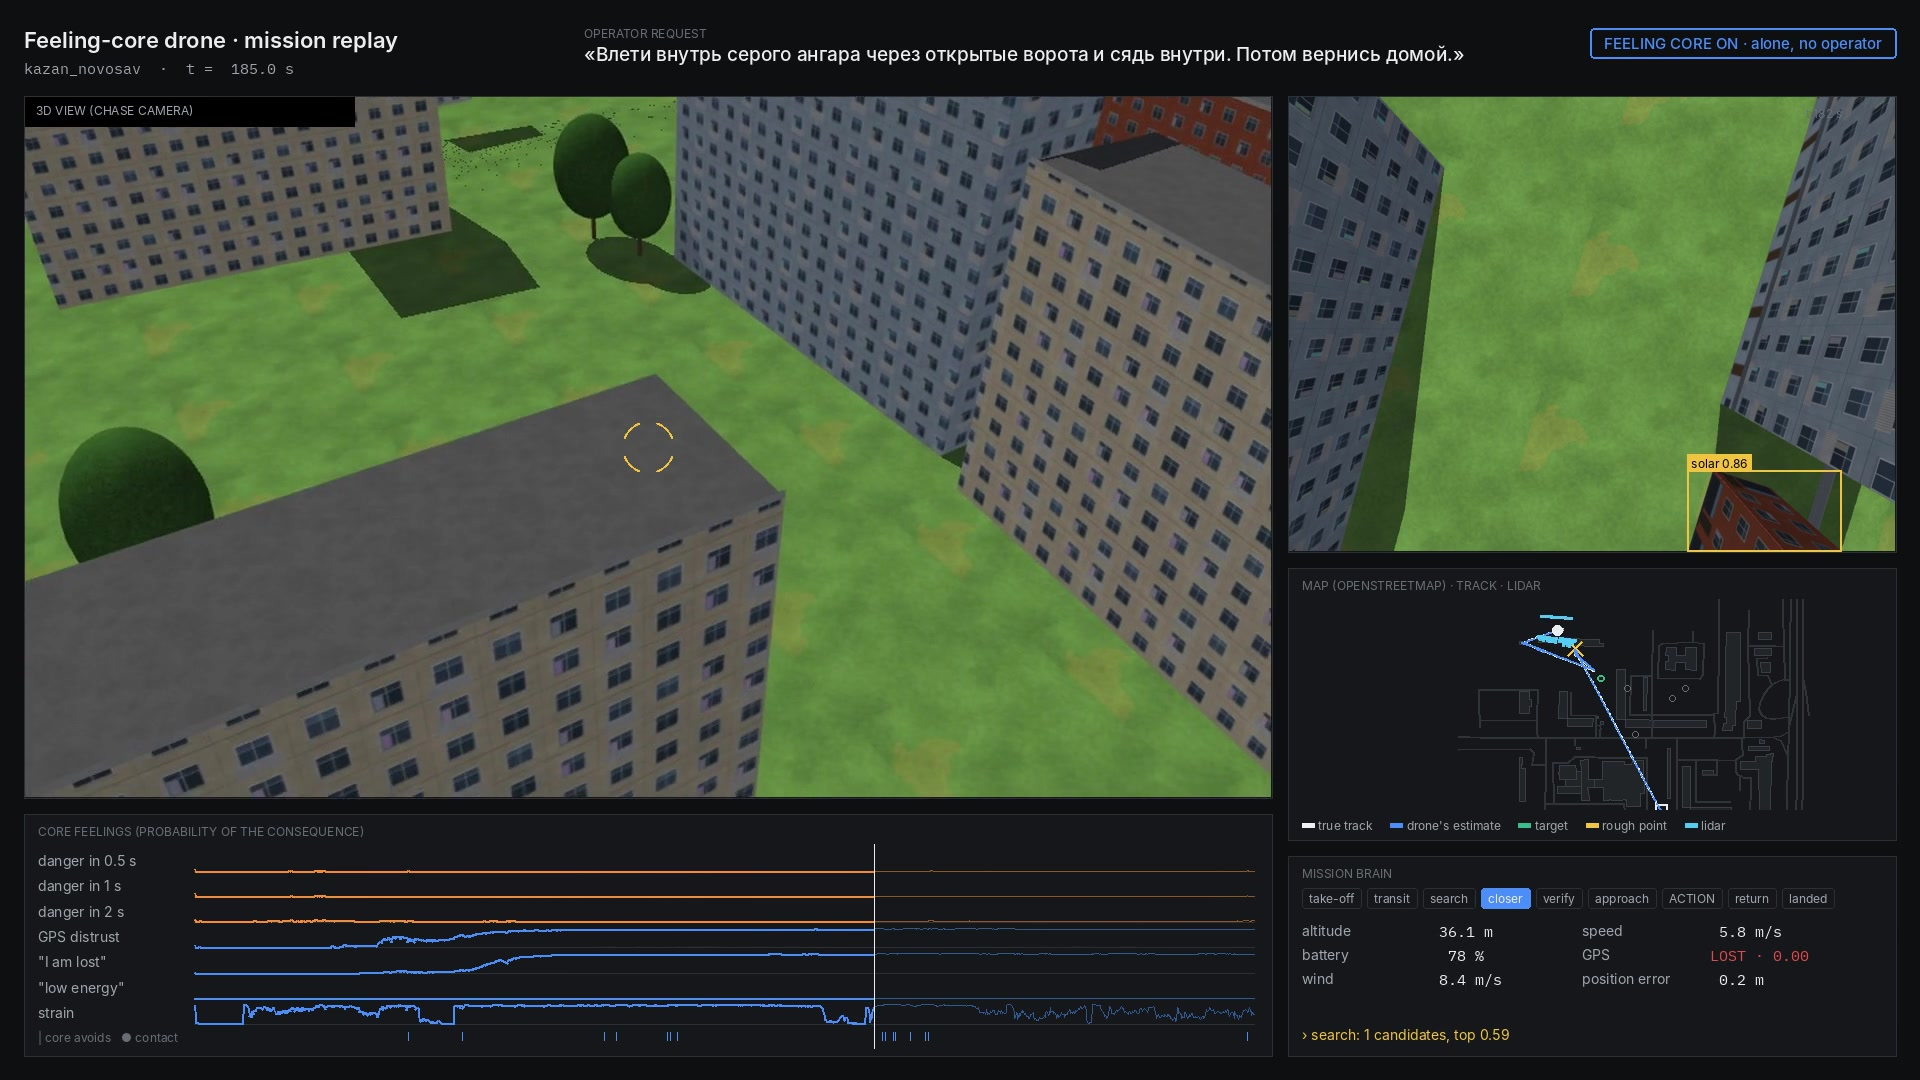
\includegraphics[width=\linewidth]{frame_mission_en.jpg}
\caption{One frame of mission G45 (enter a grey hangar, then return home) in the Kazan test district, 185\,s into the flight. GPS
was lost at 36\,s; the drone navigates on lidar and map, and its ``I am lost'' feeling has risen. Left: chase view, the core's
feelings over the whole flight, with the moments it overrode the brain. Right: the drone's camera with detections, the map with the
true track, the drone's own estimate and the rough point, and the mission brain's phase and state.}
\label{fig:frame}
\end{figure}

\begin{figure}[h]
\centering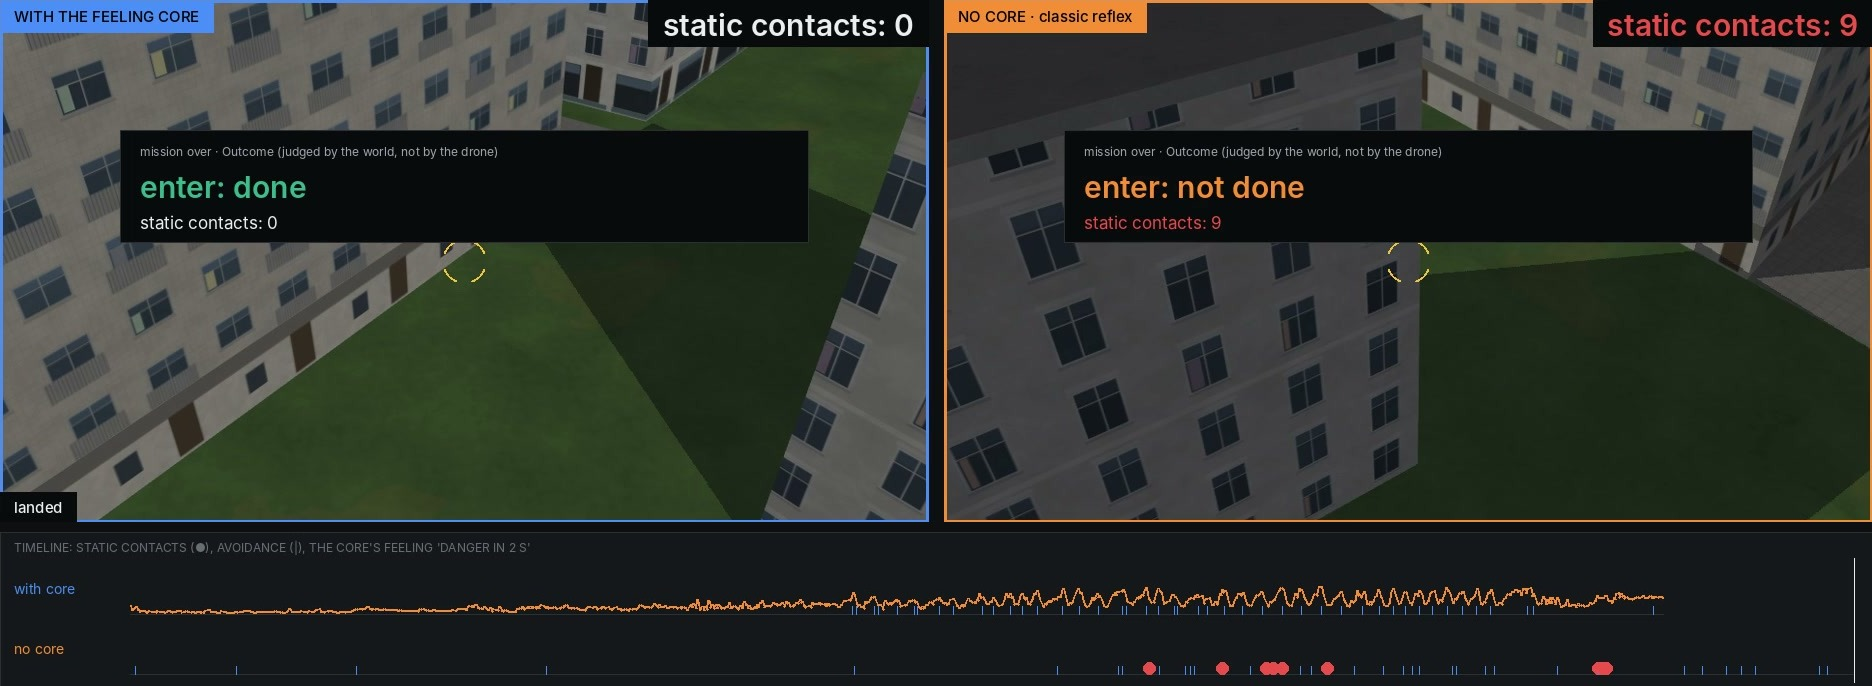
\includegraphics[width=\linewidth]{fig_compare_en.jpg}
\caption{One frame of the side-by-side video of mission G206 (enter a blue hangar, Tokyo test district): the same mission flown
with the feeling core (left) and with a classic reflex in its place (right), at the end of the mission. With the core the drone
entered the hangar without touching anything; with the reflex the entry failed after 9 static contacts. Bottom: the timeline of the
whole flight, with the static contacts of each drone (red dots) and the core's ``danger in 2\,s'' feeling. The four
side-by-side videos are replays of G2 missions run again from their plans on another GPU model; small numerical differences in the
detector change the course of a flight, so a replay differs in detail from the logged G2 flight. Over the four replays the core
had 1 static contact and the reflex 16; in one of them (G112) there was no difference, and in another (G45) the core failed the
hangar entry that the reflex made at the price of 6 contacts.}
\label{fig:compare}
\end{figure}

\begin{figure}[h]
\centering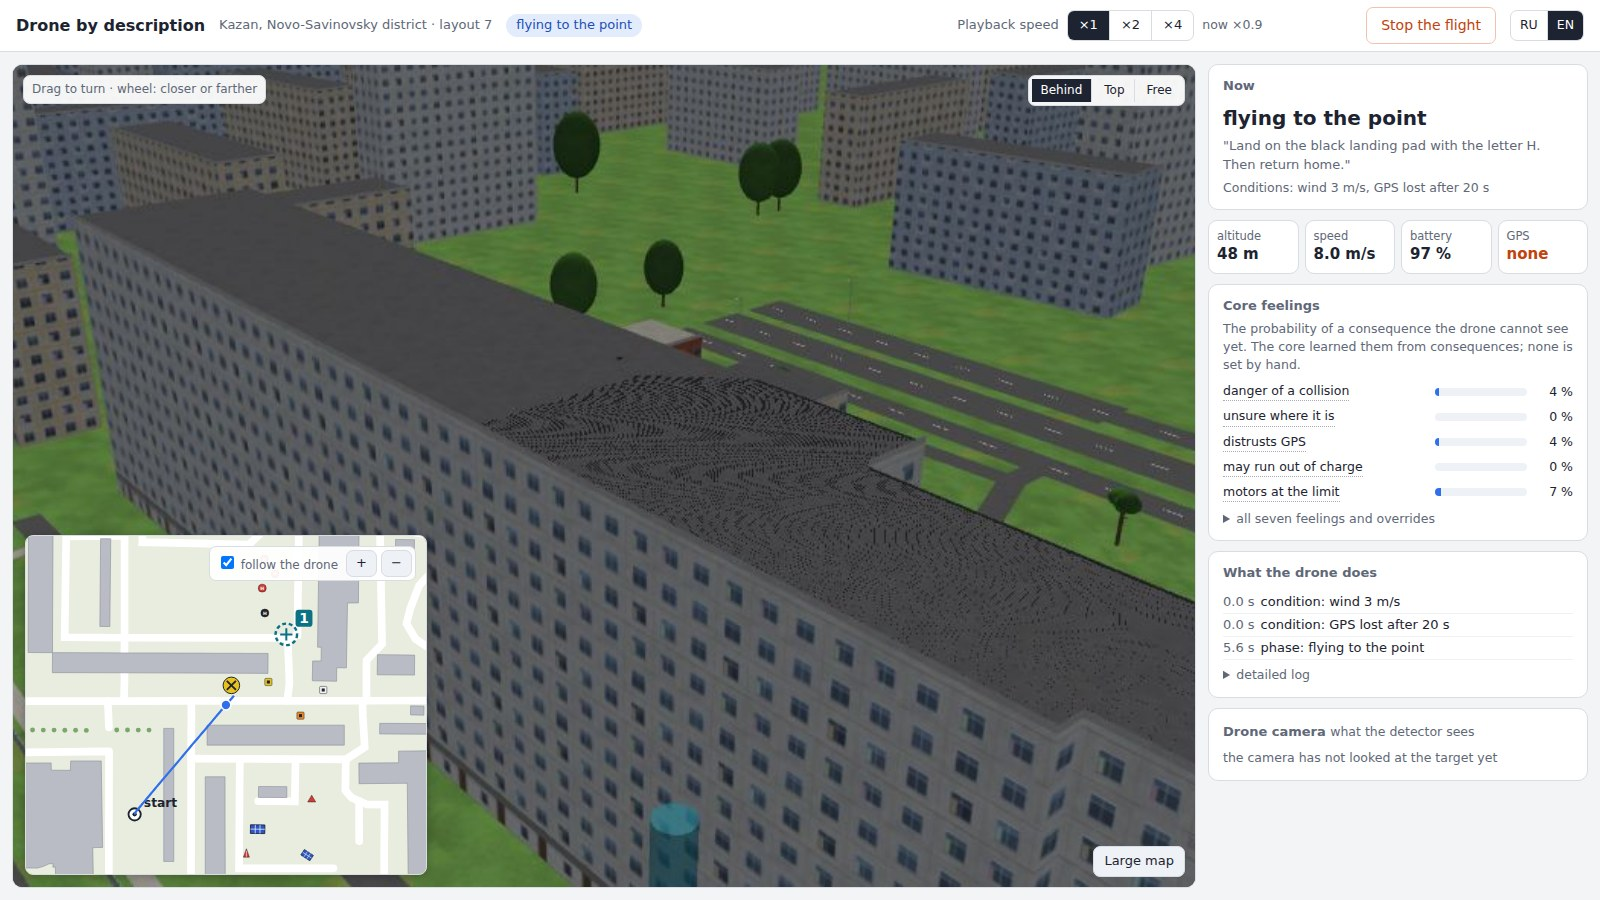
\includegraphics[width=\linewidth]{fig_app_en.jpg}
\caption{The app in flight (it has an English and a Russian interface). The large 3D chase view is rendered by the simulator itself; the map in
the corner shows the rough point, the true track and the drone's own estimate. On the right: the current phase, the conditions
(here GPS lost after 20\,s), altitude, speed, battery and GPS, five of the core's feelings and the event feed. Before the flight
the operator places a rough point, writes the request, checks the parse shown in plain words and picks the conditions.}
\label{fig:app}
\end{figure}


\end{document}
